\label{app:chap5}

Figure \ref{figapp5:px2w} displays the vision system coordinate frame, where the dotted lines mark the pixel window. The resolution of the vision system is 207$\times$315, as indicated by the corner coordinates. The pixel values of the end-effector are denoted by $(\Lambda,\Pi)$. 

The position of the $LED$ marker in pixel coordinates are given by $(\Lambda_{LED},\Pi_{LED})$


Consider the origin of the soft robot in world frame coordinates given by $(x_0,y_0)$. Note that this position can be outside of the vision system's viewing range. 

\begin{figure}[H]
    \centering
    \includegraphics[width = \textwidth]{Figures/Appendix5/pix2w.png}
    \caption{Vision system coordinate frame.}
    \label{figapp5:px2w}
\end{figure}



\begin{equation}
    \Lambda_0 = \Lambda_{LED,0} + \frac{d}{px2w} \sin(\theta_0)
\end{equation}
\begin{equation}
    \Pi_0 = \Pi_{LED,0} + \frac{d}{px2w} \cos(\theta_0)
\end{equation}


\begin{equation}
    \Lambda = \Lambda_{LED} + \frac{d}{px2w} \sin(\theta)
\end{equation}
\begin{equation}    
    \Pi = \Pi_{LED} + \frac{d}{px2w} \cos(\theta)
\end{equation}

\begin{equation}
    x = (\Lambda-\Lambda_0)px2w
\end{equation}
\begin{equation}    
    y = L - (\Pi - \Pi_0)px2w 
\end{equation}










\subsection{Ellipsoid reference tracking in simulation for relative fast trajectories}


\begin{figure}[H] 
    \begin{minipage}[b]{0.49\linewidth}
     \centering
    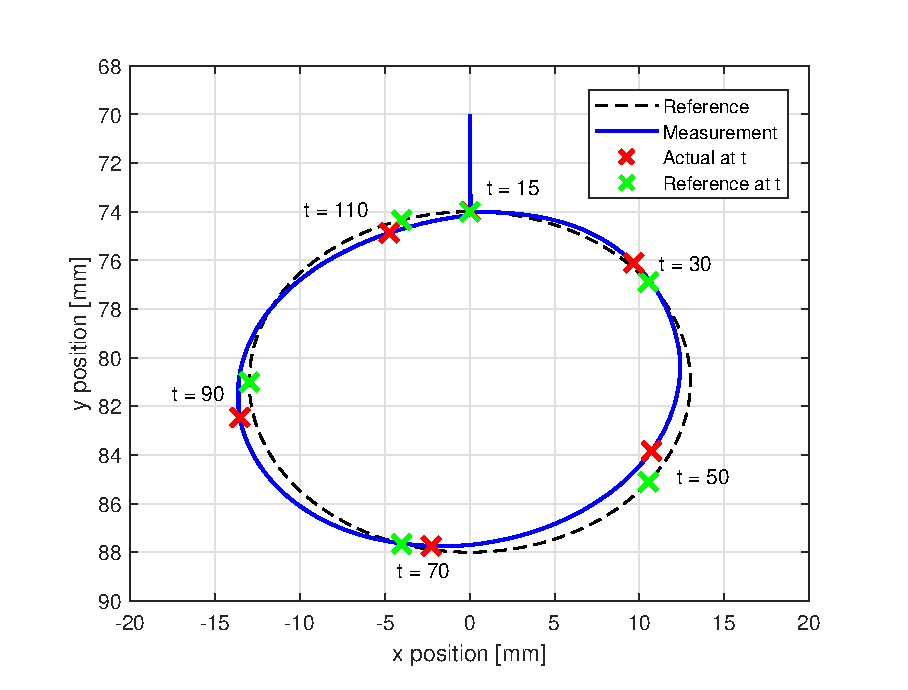
\includegraphics[width=\linewidth]{Figures/Chapter5/ellipsxy.eps} 
    \caption{Position in the x,y-plane for the ellipsoid reference path. } 
    \label{app5:xysim} 
       \end{minipage} 
    \begin{minipage}[b]{0.49\linewidth}
     \centering
    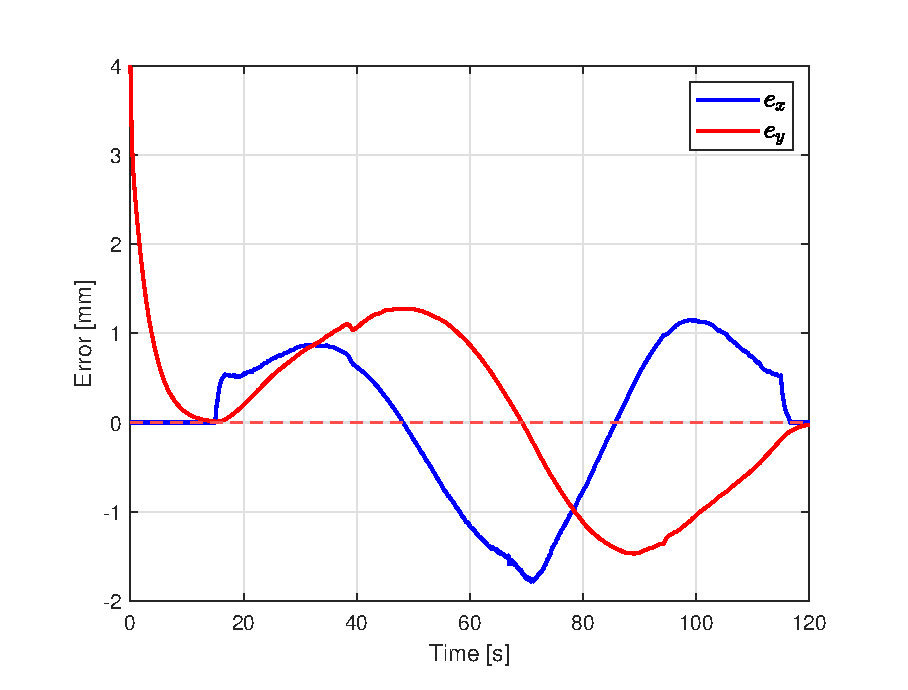
\includegraphics[width=\linewidth]{Figures/Chapter5/errorellips.eps} 
    \caption{Error in the x and y-direction as a function of time for an ellipsoid reference path.} 
    \label{app5:errorxyellipssim} 
    \end{minipage} 
\end{figure}

\begin{figure}[H]
    \centering
    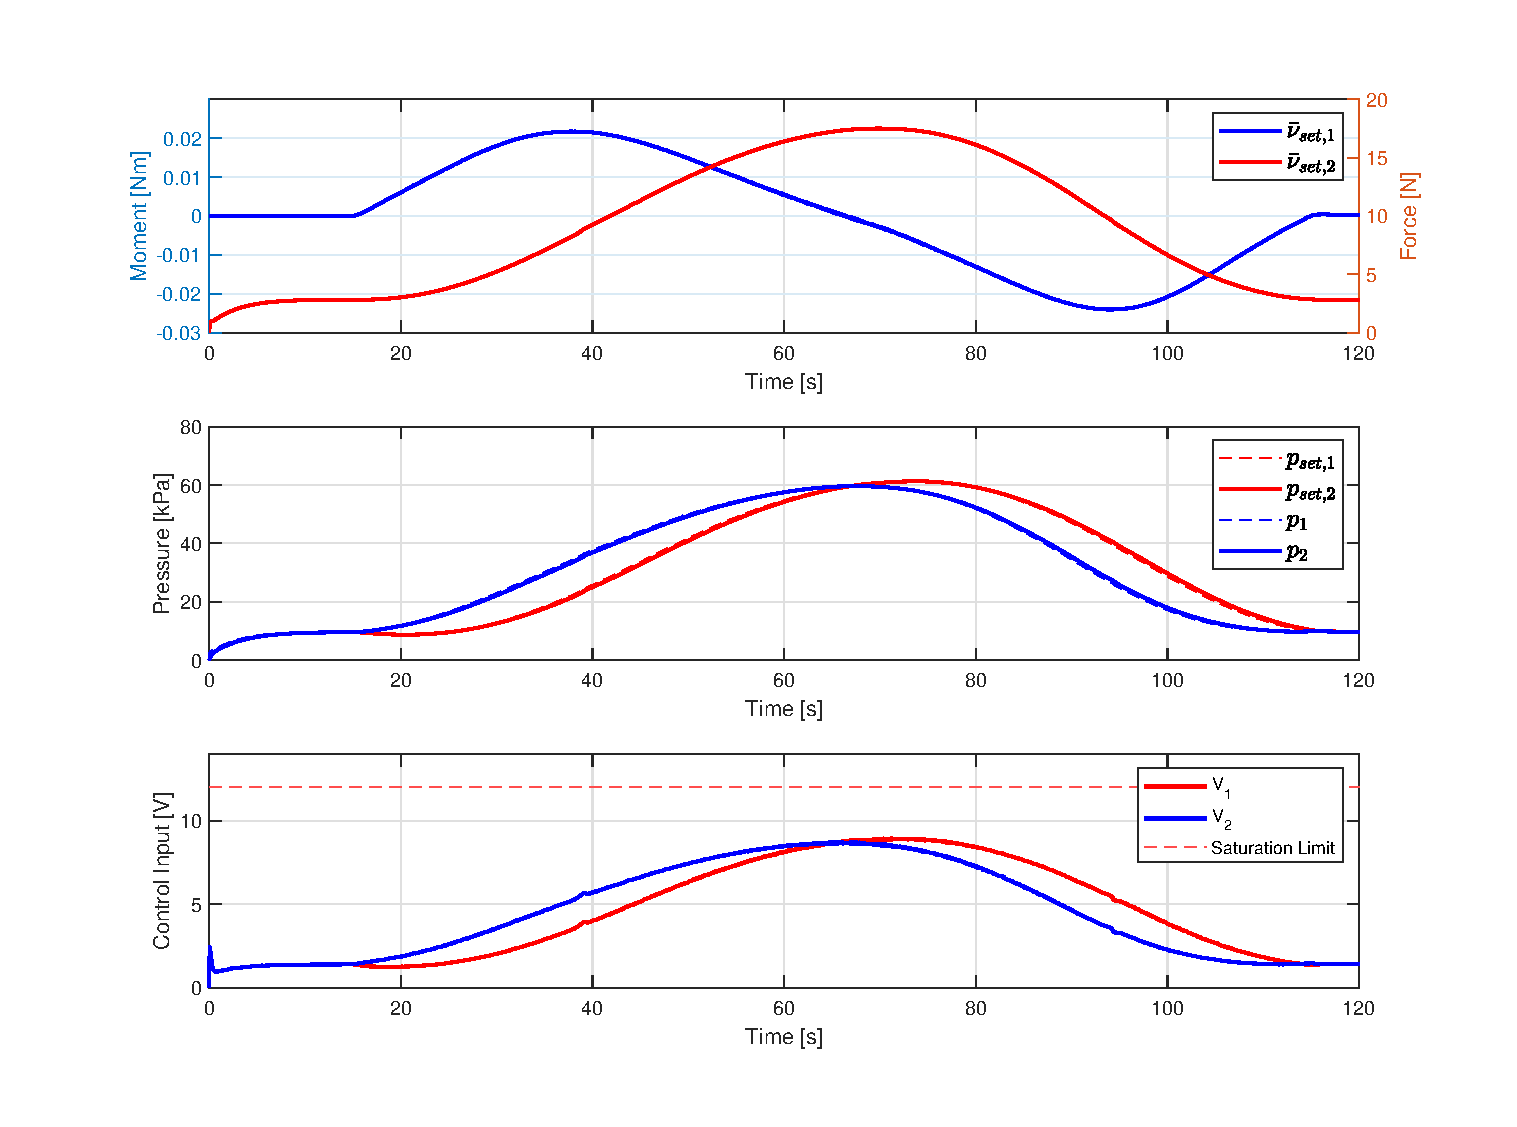
\includegraphics[width = \textwidth]{Figures/Chapter5/inputellipssim.eps}
    \caption{}
    \label{app5:controlinputellipssim}
\end{figure}
